\Subsection{Definition, use cases}

Imagine that we need to find a maximum of a function $f(x)$ in the interval $[l, r]$ but now the function is no longer monotonic. Is there a fast way (i.e. as fast as logarithmic asymptotic as in the binary search algorithm) of finding a point $x_0$ such that $f(x_0) \to \max$?

The answer is yes if our function satisfies some constraint.

\begin{definition}
    \textbf{Ternary search algorithm}

    Given a function $f(x)$ and a range $[l, r]$ in which the function is \href{https://en.wikipedia.org/wiki/Unimodality}{\underline{unimodal}} and convex, and we need to find maximum in the range (maximum for convex functions, minimum for concave functions).

    Since the function is unimodal over $[l, r]$ the following holds:

    1. $\forall a, b: l \leq a < b \leq x_0: \ f(a) < f(b)$

    2. $\forall a, b: x_0 \leq a < b \leq r: \ f(a) > f(b)$

    Where $x_0$ is a point where $f(x) = \max$

    \begin{center}
        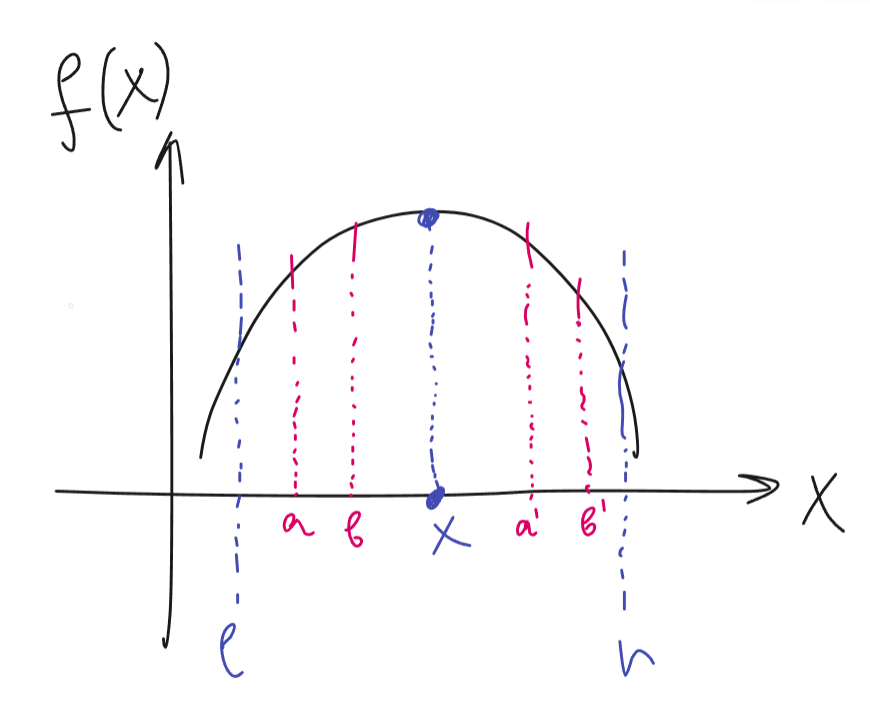
\includegraphics[scale=0.7]{./assets/09-ternary-search/1.PNG}
    \end{center}

    For the algorithm let's consider two points $m_0$ and $m_1$ such that $l < m_0 < m_1 < r$, there are several cases:

    1. $f(m_0) < f(m_1)$, then the maximum of the function $f$ cannot be located in the interval $[l, m_0]$ since there is an interval $[m_0, r]$ on which there are points where function takes greater values.

    2. $f(m_0) > f(m_1)$, then the maximum of the function $f$ cannot be located in the interval $[m_1, r]$ since the interval $[l, m_1]$ contains points in which the function takes greater values.

    3. $f(m_0) = f(m_1)$, in this case the maximum will be located in the interval $[m_0, m_1]$ but for the implementation simplisify this condition branch can be merged with any of the above.

    \begin{center}
        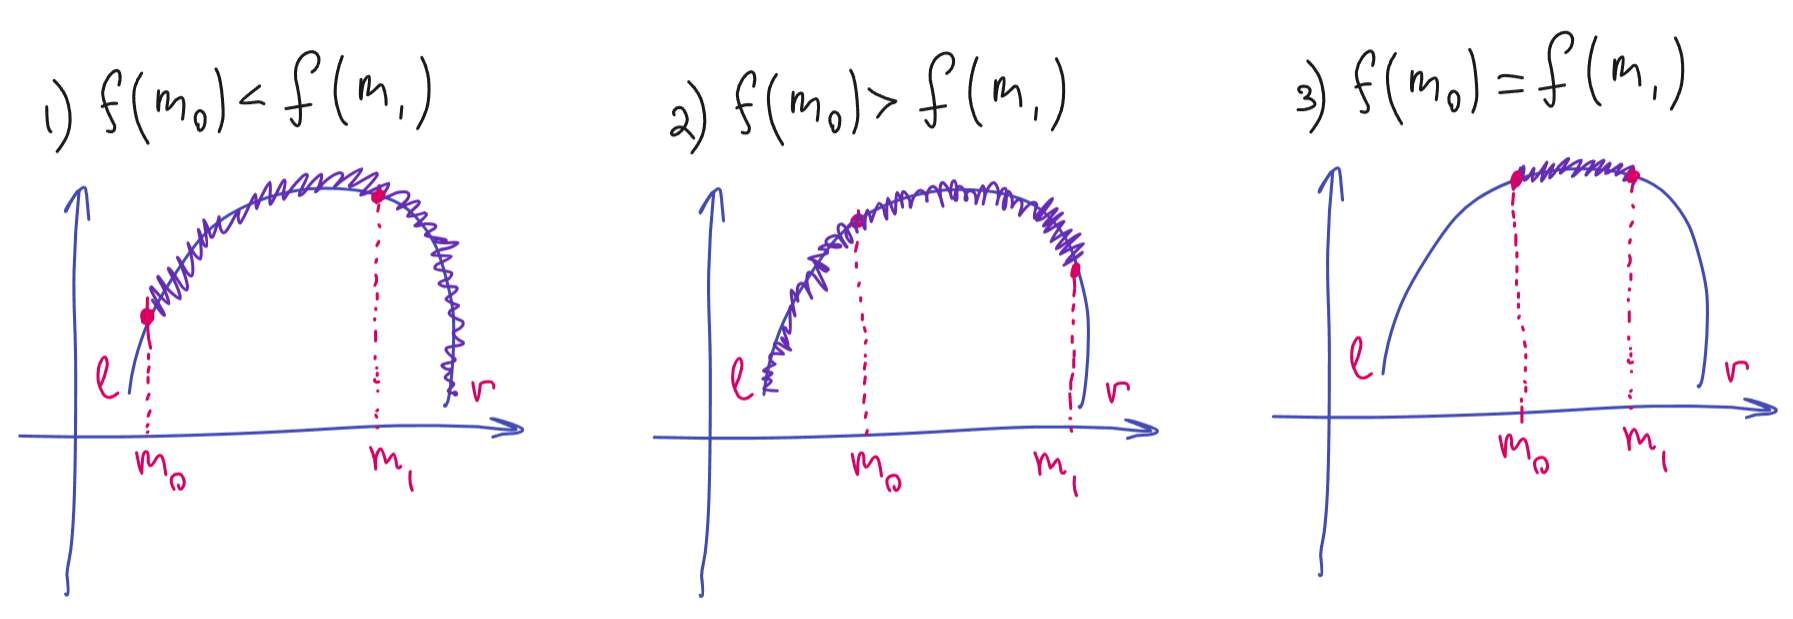
\includegraphics[scale=0.47]{./assets/09-ternary-search/2.PNG}
    \end{center}

    As for the choice of the points $m_0$ and $m_1$ we need to select something that would trancate the remaining seraching area in a manner that would give us a logarithmic asymptotic. Let's make $m_0$ be the first 3rd of the interval and $m_1$ be the second 3rd of the interval:

    1. $m_0 = l + \frac{r - l}{3}$

    2. $m_1 = l + 2 \cdot \frac{r - l}{3} = \frac{3l + 2r -2l}{3} = \frac{2r + l}{3} = \frac{3r - r + l}{3} = r - \frac{r - l}{3}$

    Notice that according to the above statement the searching interval becomes $\frac{2}{3}$ of the initial interval, thus:

    $T(n) = T(\frac{2}{3}n) + 1$

    According to \textbf{Master Theorem}:

    $a = 1, \ b = \frac{2}{3}, c = 0, \ f(n) = n^c = 1 \implies a = b^c \implies \Theta(n^c \cdot \log{n}) = \Theta(\log{n}) \implies$

    $T(n) = T(\frac{2}{3}n) + 1 = \Theta(\log{n})$

\end{definition}



\Subsection{Implementation}


Here is the implementation for a function which is an array:

\begin{lstlisting}[language=C++]
int ternary_search(vector<int>& arr) {
    // 'arr' is a unimodal function N -> Z
    int l = 0;
    int r = arr.size();

    while(r - l > 2 /* not 1 because m0 = l, m1 = r possible */) {
        int m0 = l + (r - l) / 3;
        int m1 = r - (r - l) / 3;

        if (arr[m0] < arr[m1]) {
            l = m0;
        }
        else {
            r = m1;
        }
    }

    int ans = l;

    if (r < arr.size() && arr[r] > arr[ans]) {
        ans = r;
    }

    return ans;
}
\end{lstlisting}

Here is the implementation for a function $f$ over floating-point numbers:

\begin{lstlisting}[language=C++]
int ternary_search(double l, double r, double (*f)(double)) {
    while (r - l > EPS) {
        double m0 = l + (r - l) / 3;
        double m1 = r - (r - l) / 3;

        if (f(m0) < f(m1)) {
            l = m0;
        }
        else {
            r = m1;
        }
    }

    return (l + r) / 2;
}
\end{lstlisting}
